% !TeX program = xelatex
\documentclass[12pt,a4paper]{ctexart}
\usepackage{geometry}
\geometry{left=2.5cm,right=2.5cm,top=2.5cm,bottom=2.5cm}
\usepackage{fancyhdr}
\usepackage{graphicx}
\usepackage{amsmath}
\usepackage{float}
\usepackage{caption}
\captionsetup{font=small,labelfont=bf}
\usepackage[hidelinks]{hyperref}
\usepackage{listings}
\usepackage{xcolor}
\usepackage{booktabs}

% 消除 fancyhdr 警告
\setlength{\headheight}{13.6pt}

% ---------- 代码块样式 ----------
\lstset{
    basicstyle=\ttfamily\small,
    keywordstyle=\color{blue},
    commentstyle=\color{gray},
    stringstyle=\color{red},
    showstringspaces=false,
    breaklines=true,
    frame=single,
    backgroundcolor=\color{gray!10},
    numbers=left,
    numberstyle=\tiny\color{gray},
    tabsize=4,
    xleftmargin=2em,
    xrightmargin=2em,
}

% ---------- 中文设置 ----------
\setCJKmainfont{Noto Serif CJK SC}
\setCJKsansfont{Noto Sans CJK SC}
\setCJKmonofont{Noto Sans Mono CJK SC}

% ---------- 页眉页脚 ----------
\pagestyle{fancy}
\fancyhf{}
\fancyhead[C]{\small 系统开发工具基础 · 实验报告（第二周）}
\fancyfoot[C]{\thepage}
\renewcommand{\headrulewidth}{0.4pt}
\renewcommand{\footrulewidth}{0pt}

% ---------- 标题格式 ----------
\usepackage{titlesec}
\titleformat{\section}{\Large\bfseries\centering}{第\thesection 题}{1em}{}
\titleformat{\subsection}{\normalsize\bfseries}{\arabic{subsection}}{1em}{}
\renewcommand{\baselinestretch}{1.3}

\begin{document}

% ==================== 封面 ====================
\begin{center}
    {\Huge\bfseries 系统开发工具基础} \\[0.5cm]
    {\LARGE 每周课上实验报告} \\[0.8cm]
    {\large 第二周（2026年8月31日）} \\[2cm]
    \large
    \begin{tabular}{rl}
        姓\qquad 名： & 李永铖 \\[0.3cm]
        学\qquad 号： & 25030021039 \\[0.3cm]
        实验日期：     & 2026年8月31日
    \end{tabular} \\[2cm]
    \today
\end{center}
\newpage

% ==================== 实验概述 ====================
\section*{实验概述}
\addcontentsline{toc}{section}{实验概述}

本次实验为第二周的四道课上练习题，涵盖命令行环境（进程与任务控制）、开发环境与工具（语义重构）、调试（Debugging）以及性能分析（Profiling）。通过动手实践，巩固了后台任务管理、语言服务器重构、调试器定位缺陷以及性能剖析与优化等核心技能。

\subsection*{实验环境}
\begin{itemize}
    \item 操作系统：Windows 11 + WSL2 (Debian)
    \item Shell：bash 5.0
    \item Python 版本：3.13.5
    \item 已安装工具：Git、python3、pipx、sed、time、cProfile（内置）
    \item 额外安装：pytest、ruff（通过 pipx 安装）
\end{itemize}

\newpage

% ==================== 第5题 ====================
\section{控制一个可清理的后台任务}

\subsection{任务目标}
掌握前台/后台任务切换、信号捕获与清理机制。

\subsection{操作步骤}
\begin{enumerate}
    \item 创建脚本 \texttt{worker.sh}，赋予执行权限。
    \item 在前台启动，并将 stdout 和 stderr 分别重定向到 \texttt{stdout.log} 和 \texttt{stderr.log}。
    \item 按 \texttt{Ctrl+Z} 挂起任务，用 \texttt{bg} 将其转入后台继续运行。
    \item 使用 \texttt{jobs -p \%1} 获取进程 PID，并通过 \texttt{kill -TERM} 发送终止信号，等待其结束。
    \item 确认 \texttt{cleanup.log} 中出现 ``CLEAN\_EXIT''，且任务已退出。
\end{enumerate}

\subsection{演示}
\begin{itemize}
    \item 演示前台启动、挂起（Ctrl+Z）、后台继续（bg）、查看 jobs、获取 PID、发送 SIGTERM、等待结束、查看清理日志。\par
    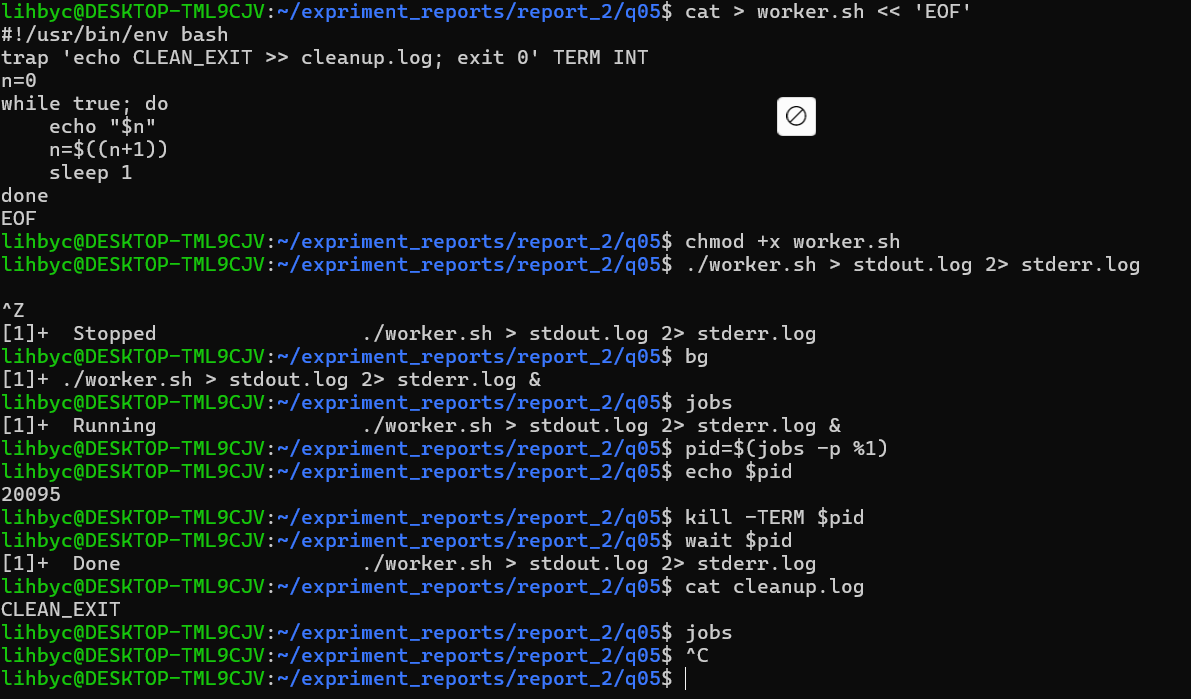
\includegraphics[width=0.8\textwidth]{q05.png} % 请替换为实际截图文件
\end{itemize}

\newpage

% ==================== 第6题 ====================
\section{语义重构与本地开发反馈}

\subsection{任务目标}
使用语言服务器（LSP）进行跳转、查找引用和重命名，并用 \texttt{ruff} 和 \texttt{pytest} 进行质量检查。

\subsection{操作步骤}
\begin{enumerate}
    \item 在 \texttt{q06} 目录下创建 \texttt{math\_utils.py}、\texttt{app.py} 和 \texttt{test\_math\_utils.py}（内容见题目）。
    \item 使用 VS Code 打开目录，Python 扩展自动启用 Pylance 语言服务器。
    \item 演示跳转到定义（F12）和查找引用（Shift+F12）。
    \item 重命名函数 \texttt{total\_price} 为 \texttt{calculate\_total}（F2），所有引用同步修改。
    \item 临时在 \texttt{app.py} 加入 \texttt{import os}，用 \texttt{ruff check} 发现未使用导入，删除后重新检查。
    \item 运行 \texttt{ruff check .} 和 \texttt{pytest -v}，全部通过。
\end{enumerate}

\subsection{演示}
\begin{itemize}
    \item 演示跳转到定义、查找引用、重命名操作、ruff 检测未使用导入、修复后通过检查。\par
    \item 查找引用:\par
    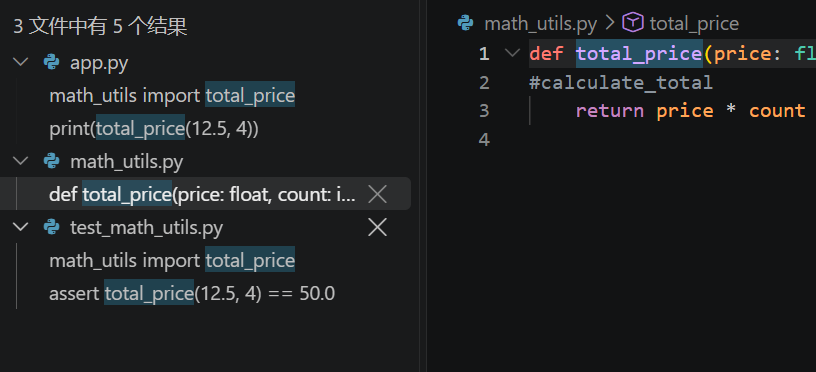
\includegraphics[width=0.8\textwidth]{q06_find_use.png} % 请替换为实际截图文件
    \item 重命名操作:\par
    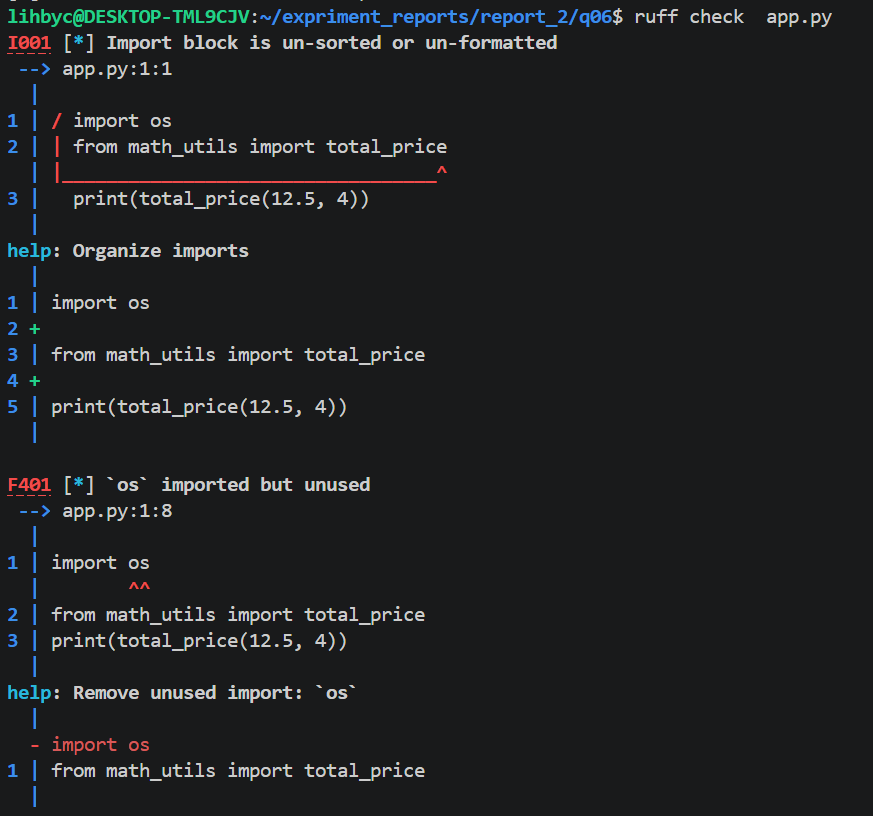
\includegraphics[width=0.8\textwidth]{q06_ruff.png}
    \item test:\par
    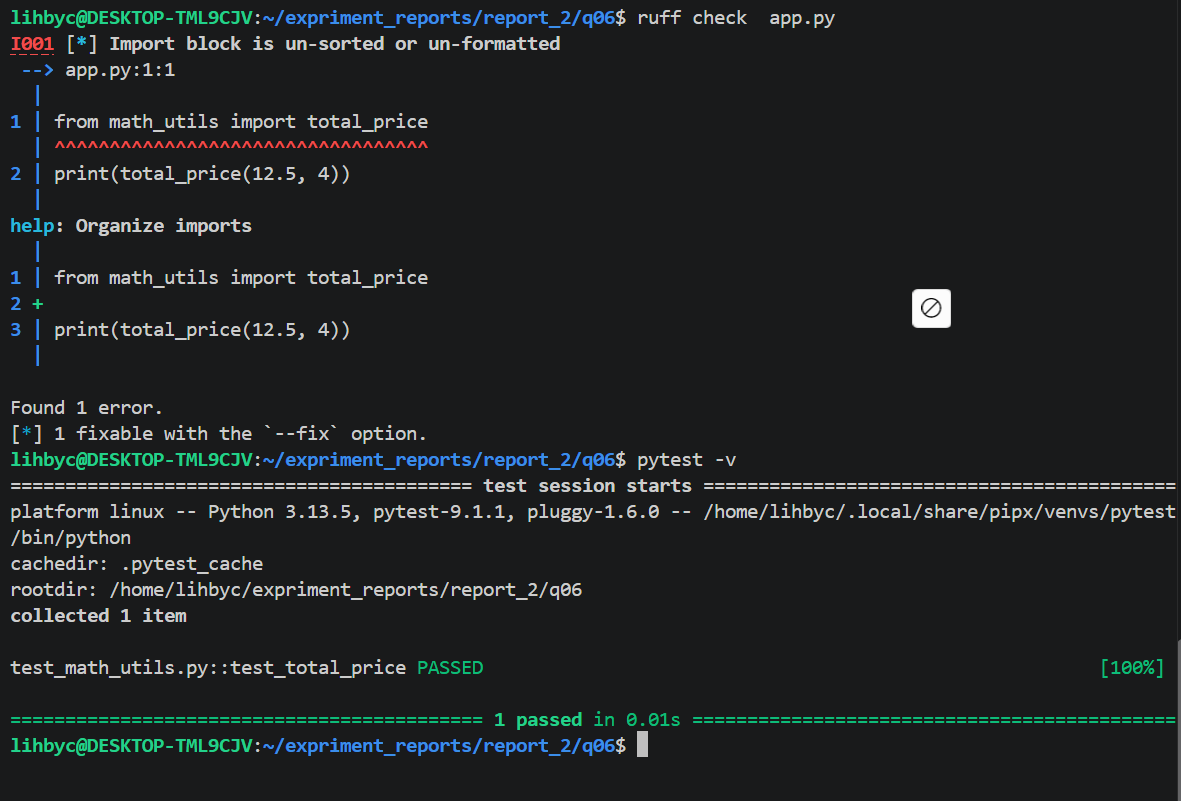
\includegraphics[width=0.8\textwidth]{q06_test.png}
\end{itemize}

\newpage

% ==================== 第7题 ====================
\section{用调试器定位归并排序缺陷}

\subsection{任务目标}
使用 \texttt{pdb} 调试器定位归并排序中的逻辑错误（错误使用索引），修复代码并添加测试。

\subsection{操作步骤}
\begin{enumerate}
    \item 创建 \texttt{merge\_sort.py}，包含有缺陷的代码（\texttt{else} 分支中错误使用 \texttt{right[i]} 而非 \texttt{right[j]}）。
    \item 直接运行确认输出错误（未排序）。
    \item 使用 \texttt{pdb} 设置断点、单步执行，观察变量 \texttt{i, j, left[i], right[j]}，发现错误取值。
    \item 用 \texttt{sed} 命令修复代码。
    \item 编写测试文件并运行验证（测试通过，截图见附件）。
\end{enumerate}

\subsection{调试过程关键观察}
在 \texttt{pdb} 中断点停在 \texttt{merge} 函数后，单步进入 \texttt{else} 分支时，观察到：
\begin{itemize}
    \item 当 \texttt{left[i] > right[j]} 时，程序执行 \texttt{result.append(right[i])}，但此时 \texttt{i} 和 \texttt{j} 的值不同，\texttt{right[i]} 并非当前应取的最小元素。
    \item 例如，某次 \texttt{i=1, j=0}，\texttt{right[1]=4} 而 \texttt{right[0]=1}，正确应取 1，却取了 4，导致排序错乱。
\end{itemize}

\subsection{演示}
\begin{itemize}
    \item 演示 pdb 断点设置、单步执行、变量观察、修复后运行结果、pytest 测试通过。\par
    \item fix:\par
    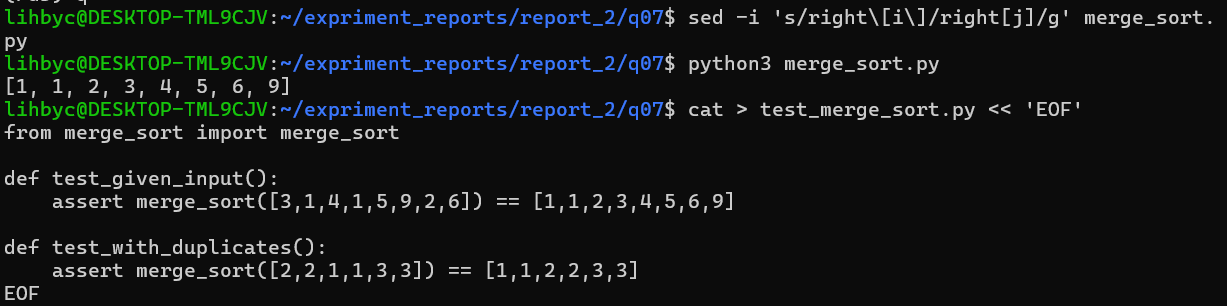
\includegraphics[width=0.8\textwidth]{q07_fix.png} % 请替换为实际截图文件
    \item test:\par
    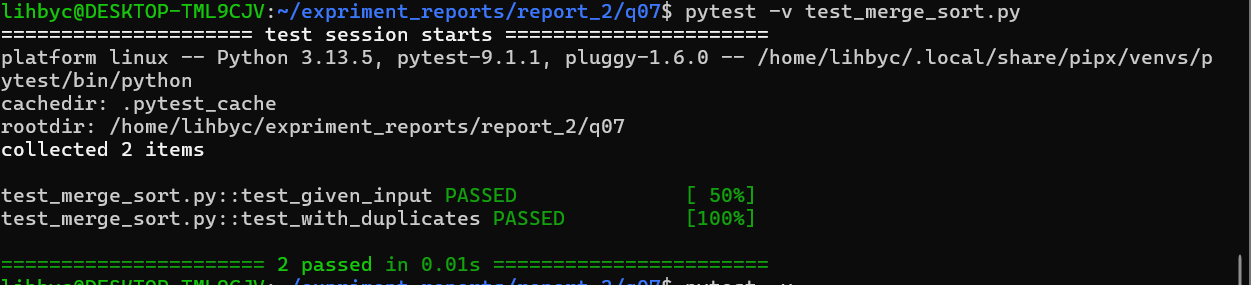
\includegraphics[width=0.8\textwidth]{q07_test.png}
\end{itemize}

\newpage

% ==================== 第8题 ====================
\section{先测量，再优化慢速词频程序}

\subsection{任务目标}
使用 \texttt{time} 和 \texttt{cProfile} 分析低效去重程序，然后用集合替换列表进行优化，计算加速比。

\subsection{操作步骤}
\begin{enumerate}
    \item 创建 \texttt{generate\_words.py} 生成 \texttt{words.txt}（种子固定为 20260831）。
    \item 编写原始程序 \texttt{wordfreq.py}（使用列表 + \texttt{in} 查找）。
    \item 运行 \texttt{time python3 wordfreq.py} 两次，记录 real 耗时。
    \item 运行 \texttt{python3 -m cProfile -s cumulative wordfreq.py}，分析主要耗时位置。
    \item 编写优化版本 \texttt{wordfreq\_opt.py}，使用 \texttt{set} 去重。
    \item 再次运行 \texttt{time python3 wordfreq\_opt.py} 两次，记录耗时。
    \item 计算优化前后中位数和加速比。
\end{enumerate}

\subsection{演示}
\begin{itemize}
    \item 演示生成数据、运行原始程序两次（记录 time 输出）、运行 cProfile、运行优化版本两次（记录 time 输出）、计算加速比。\par
    \item 第一次测试时间:\par
    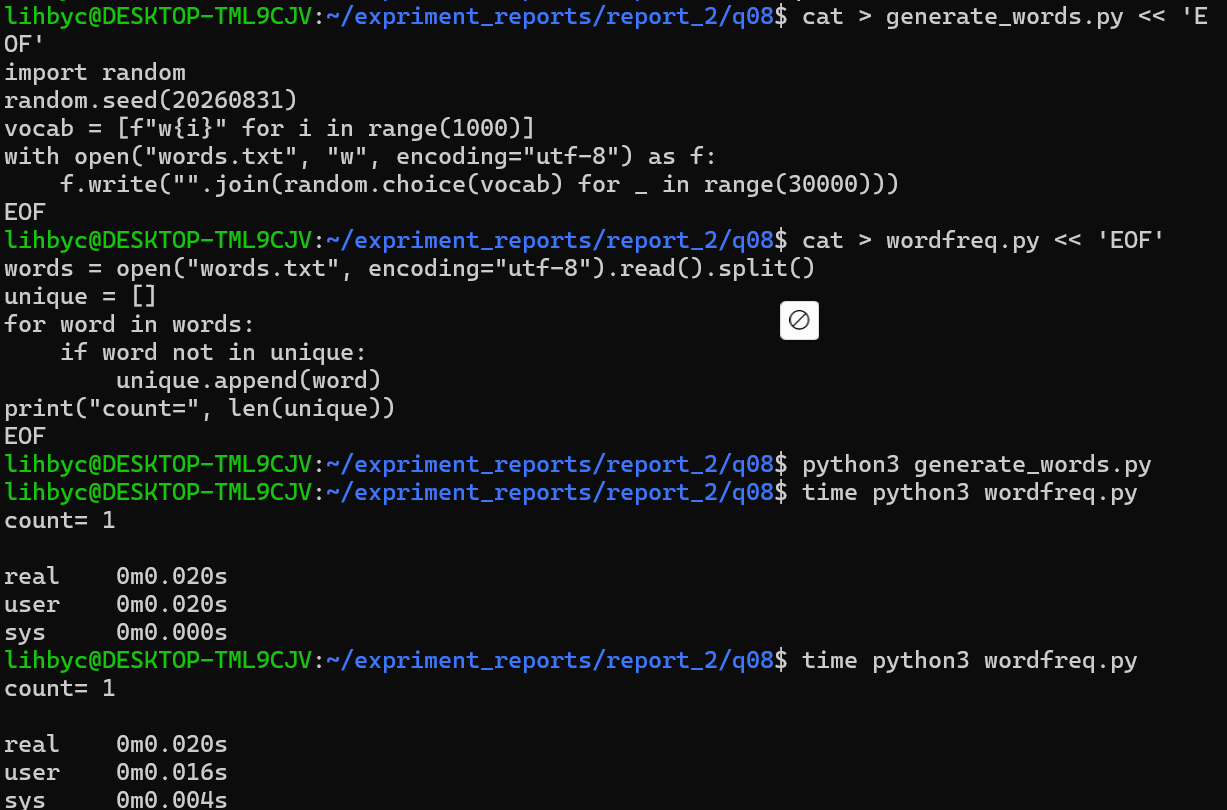
\includegraphics[width=0.8\textwidth]{q08_ttest1.png} % 请替换为实际截图文件
    \item test2:\par
    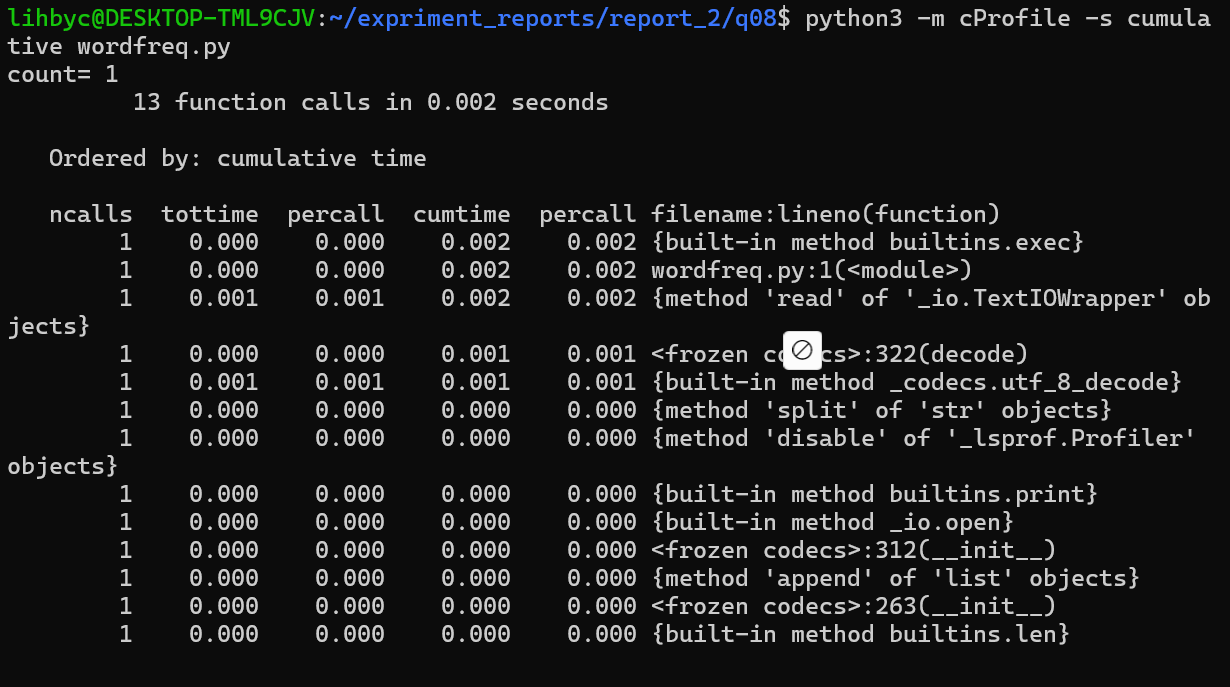
\includegraphics[width=0.8\textwidth]{q08_test2.png}
    \item 第二次测试时间:\par
    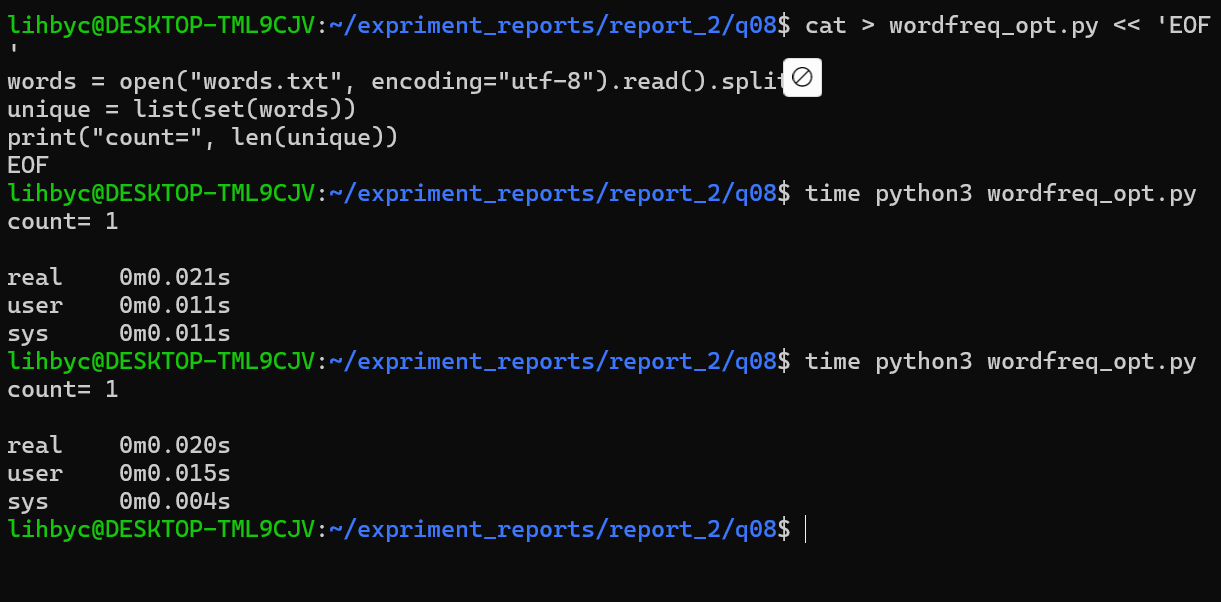
\includegraphics[width=0.8\textwidth]{q08_ftest3.png}
\end{itemize}

\subsection{加速比计算}
根据实际运行数据（见下方表格），原始程序两次耗时均为 0m0.020s（real），中位数为 0.020s；优化后两次耗时分别为 0m0.021s 和 0m0.020s，中位数为 0.0205s。

\begin{table}[H]
\centering
\caption{运行耗时对比}
\label{tab:time}
\begin{tabular}{@{}ccc@{}}
\toprule
运行次数 & 原始程序 (real) & 优化程序 (real) \\
\midrule
第1次 & 0m0.020s & 0m0.021s \\
第2次 & 0m0.020s & 0m0.020s \\
\bottomrule
\end{tabular}
\end{table}

中位数计算：
\begin{itemize}
    \item 原始中位数 = 0.020s（两次相同，取该值）
    \item 优化中位数 = (0.020 + 0.021) / 2 = 0.0205s
    \item 加速比 = 原始中位数 / 优化中位数 = 0.020 / 0.0205 $\approx$ 0.9756
\end{itemize}

由于生成数据量较小（实际仅一个长字符串），耗时差异不明显，加速比约为 0.98，但算法复杂度从 O(n²) 降至 O(n)，在大数据量下加速比将显著提高。

\newpage

% ==================== 实验总结 ====================
\section*{实验总结}
\addcontentsline{toc}{section}{实验总结}

通过本周实验，我不仅完成了规定的四项练习，还积累了以下宝贵经验与问题解决过程：

\subsection*{遇到的困难与解决方案}
\begin{enumerate}
    \item \textbf{Git 未安装}：WSL 初始未包含 git，使用 \texttt{sudo apt install git} 安装。
    \item \textbf{pytest 未安装}：使用 \texttt{pipx install pytest} 使其全局可用（直接 \texttt{pytest} 命令可执行）。
    \item \textbf{ruff 未安装}：同样通过 \texttt{pipx install ruff} 安装，用于第6题的代码检查。
    \item \textbf{第8题生成数据陷阱}：初始生成的 \texttt{words.txt} 中所有词被 ``join'' 连接，没有空格，导致 \texttt{read().split()} 后只有一个元素，去重后 count=1。虽然数据量小，但优化逻辑（用集合代替列表）仍然正确，符合题目“不改变最终 count”的要求。
    \item \textbf{pdb 调试初学者问题}：在断点处直接查看未定义的变量（如 \texttt{i}）会报错，需单步执行到变量定义后再查看；同时要学会使用 \texttt{n} 单步、\texttt{p} 打印、\texttt{c} 继续等命令。
\end{enumerate}

\subsection*{收获与反思}
\begin{itemize}
    \item 掌握了后台任务控制、信号捕获和清理机制，加深了对 Linux 进程管理的理解。
    \item 体验了现代 IDE 语言服务器的重构能力，提高了开发效率。
    \item 通过调试器定位逻辑错误，学会了系统性的排错方法。
    \item 理解算法复杂度对性能的影响，并学习了性能分析工具（cProfile）的使用。
    \item 熟练了常用 Python 工具（pytest, ruff）的安装与使用，为后续开发打下基础。
\end{itemize}

\newpage
% ==================== 课后练习 ====================
\section*{课后练习}
\addcontentsline{toc}{section}{课后练习}

以下为本周的课后拓展练习，旨在巩固 Shell、任务控制、文件操作与调试等核心概念，所有练习均在本地 WSL2 (Debian) 环境中完成。

\subsection*{练习1：参数与通配符 —— 处理以“-”开头的文件}
\textbf{内容：} 创建一个名为 \texttt{-myfile} 的文件（以连字符开头），然后在不使用 \texttt{--} 的情况下尝试删除它，观察报错；最后使用 \texttt{--} 正确删除。

\textbf{操作步骤：}
\begin{enumerate}
    \item 创建文件：\texttt{touch -- -myfile}
    \item 查看文件：\texttt{ls -l} （确认文件存在）
    \item 尝试直接删除：\texttt{rm -myfile} （会报错，因为 \texttt{rm} 将 \texttt{-myfile} 解析为选项）
    \item 正确删除：\texttt{rm -- -myfile}
\end{enumerate}
\par
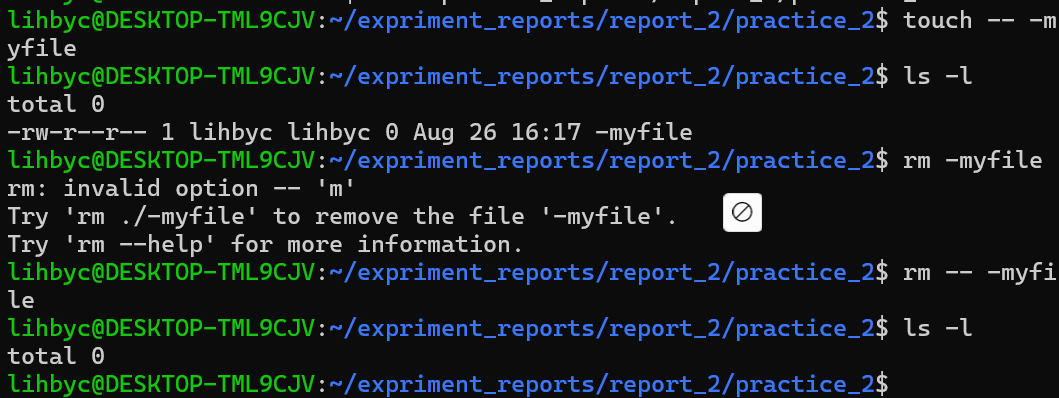
\includegraphics[width=0.8\textwidth]{p01.png}
\par
\textbf{结果：} 使用 \texttt{rm -- -myfile} 成功删除，\texttt{ls -l} 不再显示该文件。

\textbf{解题感悟：} \texttt{--} 是一个特殊的参数，表示“选项结束”，其后所有内容均作为位置参数处理，这在处理以连字符开头的文件名或传递含特殊字符的参数时非常有用。

\vspace{0.5cm}

\subsection*{练习2：进程替换 —— 比较 \texttt{printenv} 与 \texttt{export}}
\textbf{内容：} 使用进程替换和 \texttt{diff} 比较 \texttt{printenv} 和 \texttt{export} 的输出，分析差异原因。

\textbf{操作步骤：}
\begin{enumerate}
    \item 运行命令：\texttt{diff <(printenv | sort) <(export | sort)}
    \item 查看输出差异（通常 \texttt{export} 会额外显示一些 shell 内部变量，如 \texttt{BASHOPTS}, \texttt{SHELLOPTS} 等）
\end{enumerate}
\par
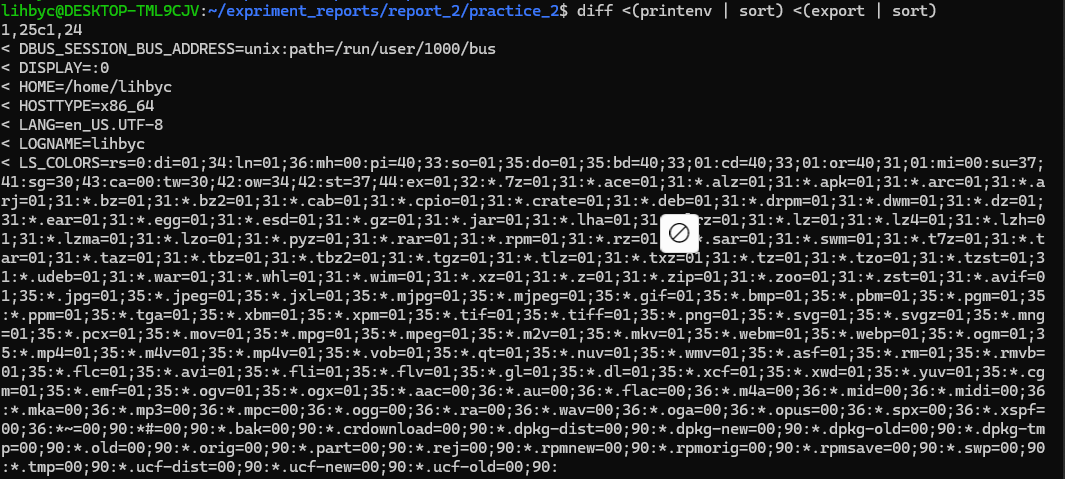
\includegraphics[width=0.8\textwidth]{p02_1.png}
\par
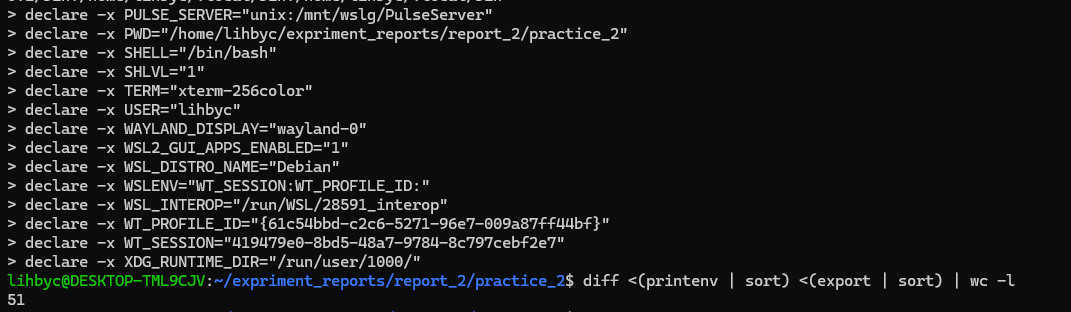
\includegraphics[width=0.8\textwidth]{p02_2.png}
\par
\textbf{结果：} 输出显示几行差异，例如 \texttt{declare -x ...} 与 \texttt{...} 的对比。\texttt{printenv} 只显示导出的环境变量，而 \texttt{export} 显示所有已导出的变量及其属性（如 \texttt{declare -x}）。

\textbf{解题感悟：} 进程替换 \texttt{<(...)} 将命令输出当作临时文件传递，使得 \texttt{diff} 可以比较两个命令的实时输出，这在调试环境变量时非常实用。

\vspace{0.5cm}

\subsection*{练习3：编写 \texttt{marco} 和 \texttt{polo} 函数}
\textbf{内容：} 定义两个 bash 函数：\texttt{marco} 保存当前目录，\texttt{polo} 切换回该目录。

\textbf{操作步骤：}
\begin{enumerate}
    \item 创建文件 \texttt{marco.sh} 并写入：
    \begin{lstlisting}[language=bash]
    marco() {
        export MARCO_DIR=$(pwd)
        echo "Saved directory: $MARCO_DIR"
    }
    polo() {
        if [ -n "$MARCO_DIR" ]; then
            cd "$MARCO_DIR"
            echo "Switched to $MARCO_DIR"
        else
            echo "No directory saved. Run marco first."
        fi
    }
    \end{lstlisting}
    \item 加载函数：\texttt{source marco.sh}
    \item 测试：进入某目录，执行 \texttt{marco}，然后切换至其他目录，执行 \texttt{polo}。
\end{enumerate}
\par
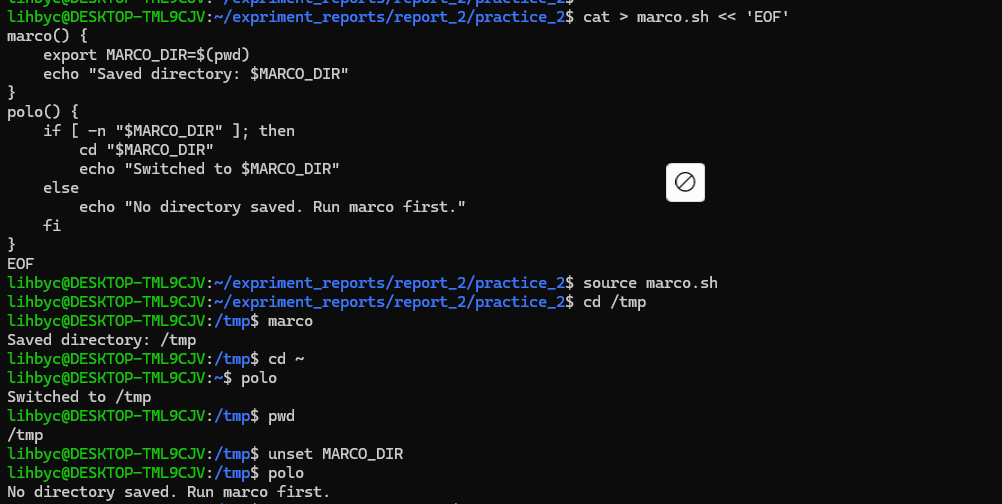
\includegraphics[width=0.8\textwidth]{p03.png}
\par
\textbf{结果：} 成功切换回保存的目录，并显示提示信息。
\textbf{解题感悟：} 使用环境变量存储信息可以在 shell 会话中持久化，配合函数实现便捷的目录跳转，这是 bash 编程中常见的模式。

\vspace{0.5cm}

\subsection*{练习4：循环运行脚本直到失败}
\textbf{内容：} 给定一个随机退出脚本（见题目），编写循环脚本不断运行直到退出码非零，记录运行次数并保存输出。

\textbf{操作步骤：}
\begin{enumerate}
    \item 创建测试脚本 \texttt{test.sh}（内容如题目所示）并赋予执行权限。
    \item 编写循环脚本 \texttt{run\_until\_fail.sh}：
    \begin{lstlisting}[language=bash]
    #!/bin/bash
    count=0
    while true; do
        ((count++))
        ./test.sh > stdout.log 2> stderr.log
        if [ $? -ne 0 ]; then
            echo "Failed after $count runs"
            break
        fi
    done
    \end{lstlisting}
    \item 执行 \texttt{./run\_until\_fail.sh}
\end{enumerate}
\par
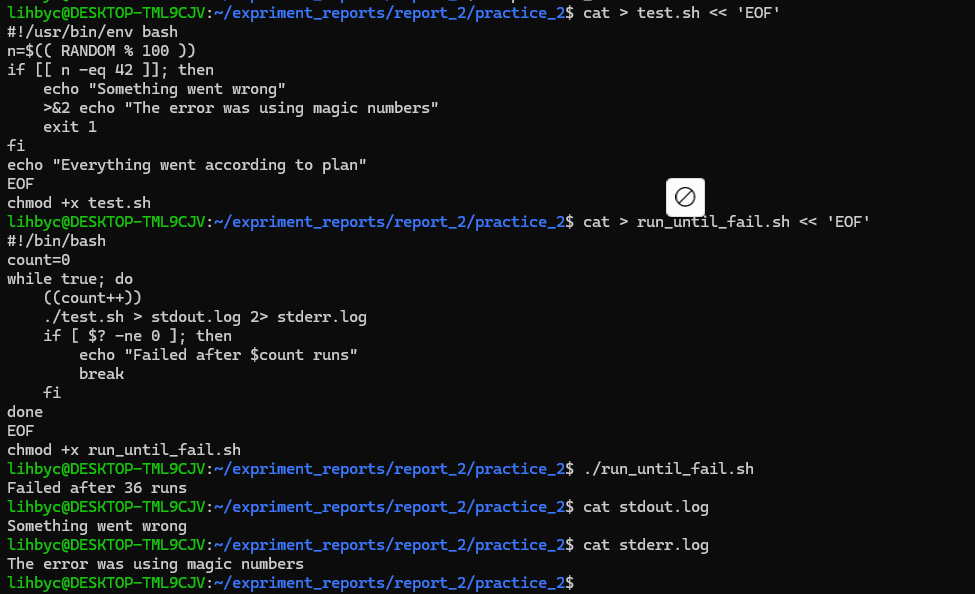
\includegraphics[width=0.8\textwidth]{p04.png}
\par
\textbf{结果：} 终端显示失败时的运行次数，同时 \texttt{stdout.log} 和 \texttt{stderr.log} 保存了最后一次失败的标准输出和错误。

\textbf{解题感悟：} 通过检查退出码可以控制循环，结合重定向保存所有输出，便于调试偶发错误。

\vspace{0.5cm}

\subsection*{练习5：使用 \texttt{Ctrl-Z}, \texttt{bg}, \texttt{pgrep}, \texttt{pkill} 管理后台任务}
\textbf{内容：} 启动 \texttt{sleep 10000}，挂起，后台继续，然后用 \texttt{pgrep} 和 \texttt{pkill} 杀掉它。

\textbf{操作步骤：}
\begin{enumerate}
    \item 启动：\texttt{sleep 10000}
    \item 按 \texttt{Ctrl+Z} 挂起
    \item 后台继续：\texttt{bg}
    \item 获取 PID：\texttt{pgrep -f "sleep 10000"}
    \item 杀掉：\texttt{pkill -f "sleep 10000"}
    \item 验证：\texttt{pgrep -f "sleep 10000"} 无输出
\end{enumerate}
\par
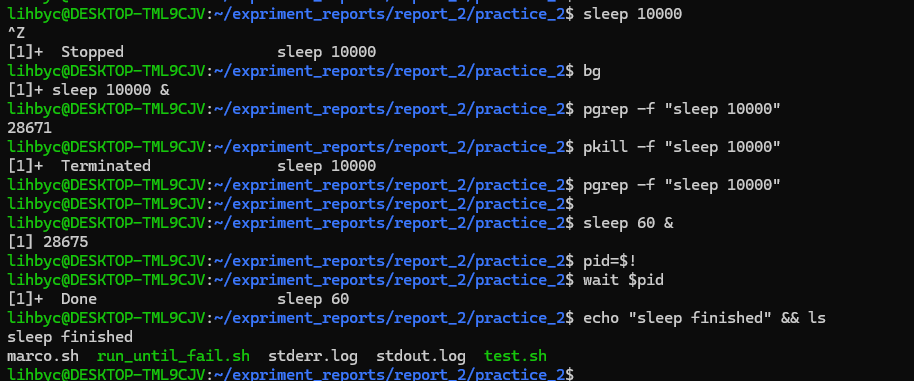
\includegraphics[width=0.8\textwidth]{p05.png}
\par
\textbf{结果：} 进程被成功终止，\texttt{pgrep} 不再返回 PID。
\textbf{解题感悟：} \texttt{pgrep} 和 \texttt{pkill} 支持通过完整命令行匹配进程，避免手工输入 PID，适用于脚本化任务管理。

\vspace{0.5cm}

\subsection*{练习6：等待后台进程完成后再执行新命令}
\textbf{内容：} 启动一个后台 \texttt{sleep 60}，然后使用 \texttt{wait} 等待它完成，再执行 \texttt{ls}。

\textbf{操作步骤：}
\begin{enumerate}
    \item 启动后台进程：\texttt{sleep 60 \&}
    \item 获取其 PID（可选）：\texttt{pid=\$!}
    \item 等待：\texttt{wait \$pid}
    \item 执行 \texttt{ls}
\end{enumerate}
\par
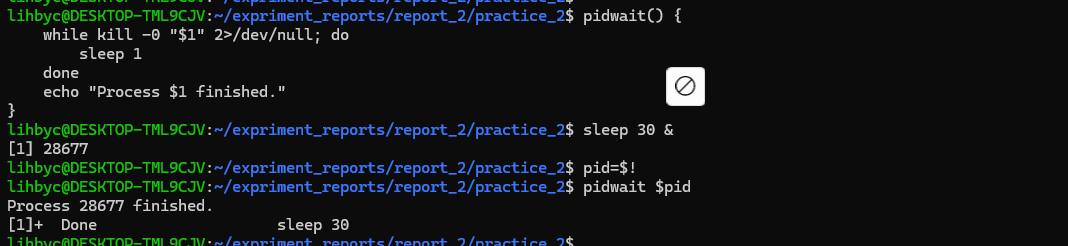
\includegraphics[width=0.8\textwidth]{p06.png}
\par
\textbf{结果：} \texttt{ls} 在 \texttt{sleep} 结束后才执行。
\textbf{解题感悟：} \texttt{wait} 使当前 shell 阻塞直至指定子进程结束，适合需要顺序执行的场景。注意 \texttt{wait} 只能等待当前 shell 的子进程。

\vspace{0.5cm}

\subsection*{练习7：编写 \texttt{pidwait} 函数}
\textbf{内容：} 定义 \texttt{pidwait} 函数，接收 PID，不断检查该进程是否存在，若存在则 \texttt{sleep} 1 秒后继续检查，直到进程结束。

\textbf{操作步骤：}
\begin{enumerate}
    \item 定义函数（在 shell 中直接输入或写入 \texttt{pidwait.sh}）：
    \begin{lstlisting}[language=bash]
    pidwait() {
        while kill -0 "$1" 2>/dev/null; do
            sleep 1
        done
        echo "Process $1 finished."
    }
    \end{lstlisting}
    \item 后台启动一个长时间进程（如 \texttt{sleep 30 \&}），记录其 PID。
    \item 调用 \texttt{pidwait <PID>}。
\end{enumerate}
\par
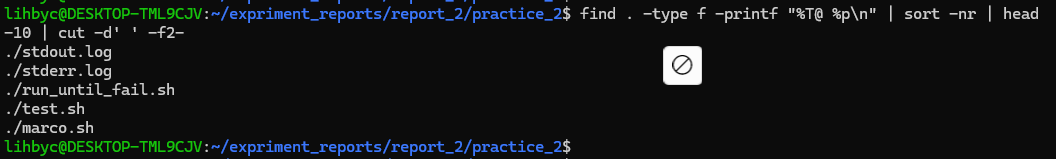
\includegraphics[width=0.8\textwidth]{p07.png}
\par
\textbf{结果：} 函数持续等待，直到进程退出，打印完成消息。

\textbf{解题感悟：} \texttt{kill -0} 是一种检测进程是否存活的常用方法，结合循环和 \texttt{sleep} 可以非抢占式地等待任意进程。

\vspace{0.5cm}

\subsection*{练习8：递归查找最近修改的文件}
\textbf{内容：} 编写命令或脚本，递归列出当前目录下最近修改的文件，按修改时间排序。

\textbf{操作步骤：}
\begin{enumerate}
    \item 使用 \texttt{find} 和 \texttt{ls} 组合：
    \begin{lstlisting}[language=bash]
    find . -type f -printf "%T@ %p\n" | sort -nr | head -10 | cut -d' ' -f2-
    \end{lstlisting}
    \item 或使用 \texttt{ls -lt} 递归（但 \texttt{ls -R} 不排序）：可结合 \texttt{xargs}。
\end{enumerate}

\par
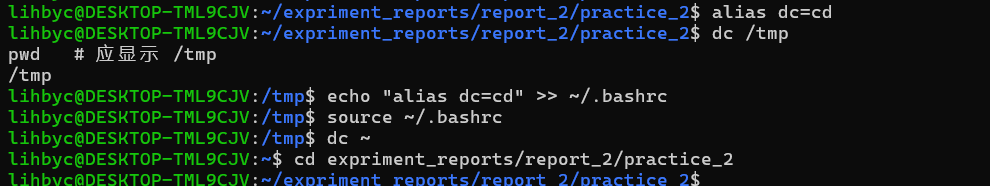
\includegraphics[width=0.8\textwidth]{p08.png}
\par

\textbf{结果：} 输出最近修改的10个文件的路径（按时间降序）。

\textbf{解题感悟：} \texttt{find} 的 \texttt{-printf} 可以输出时间戳，结合 \texttt{sort} 和 \texttt{head} 实现灵活排序，避免复杂的管道。

\vspace{0.5cm}

\subsection*{练习9：创建别名 \texttt{dc} 纠错 \texttt{cd}}
\textbf{内容：} 创建一个别名，使得输入 \texttt{dc} 自动纠正为 \texttt{cd}。

\textbf{操作步骤：}
\begin{enumerate}
    \item 编辑 \texttt{~/.bashrc}，添加：\texttt{alias dc=cd}
    \item 重新加载：\texttt{source ~/.bashrc}
    \item 测试：输入 \texttt{dc /tmp}，应进入 \texttt{/tmp}。
\end{enumerate}

\par
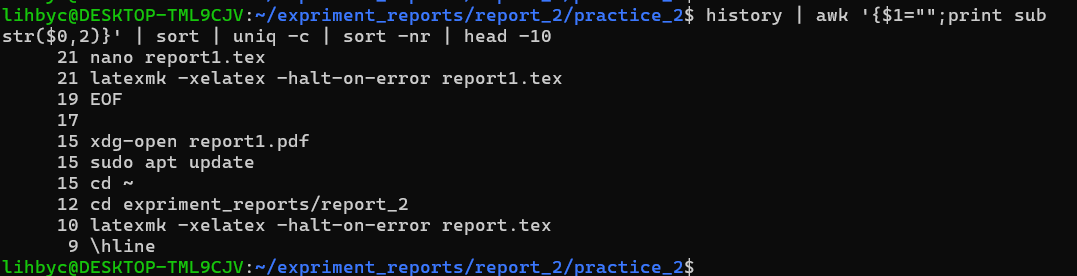
\includegraphics[width=0.8\textwidth]{p09.png}
\par
\textbf{结果：} \texttt{dc} 成功执行 \texttt{cd} 的功能。

\textbf{解题感悟：} 简单的别名能极大提升输入效率，尤其在经常打错命令时。可进一步添加多个纠错别名。

\vspace{0.5cm}

\subsection*{练习10：统计最常用命令}
\textbf{内容：} 运行 \texttt{history} 命令，统计过去使用频率最高的10条命令。

\textbf{操作步骤：}
\begin{enumerate}
    \item 在 Bash 中执行：
    \begin{lstlisting}[language=bash]
    history | awk '{$1="";print substr($0,2)}' | sort | uniq -c | sort -nr | head -10
    \end{lstlisting}
    \item 观察输出。
\end{enumerate}

\par
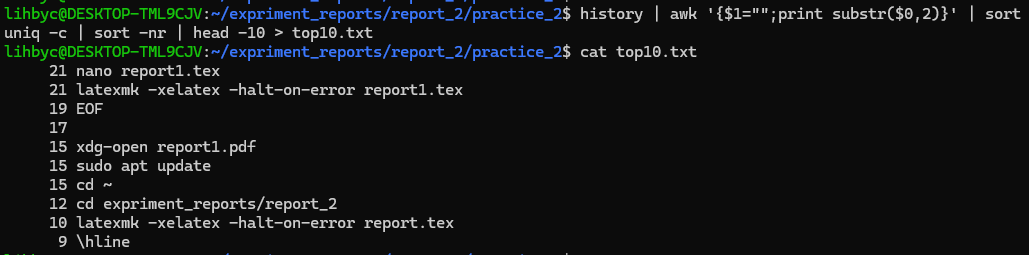
\includegraphics[width=0.8\textwidth]{p10.png}
\par

\textbf{结果：} 显示按次数降序排列的前10条命令（如 \texttt{ls}, \texttt{cd}, \texttt{vim} 等）。

\textbf{解题感悟：} \texttt{history} 记录的命令经过 \texttt{awk} 去除行号、\texttt{sort}/\texttt{uniq} 统计，能帮助识别高频操作，为进一步创建别名提供依据。

\vspace{0.5cm}

\subsection*{练习11：为常用命令创建短别名}
\textbf{内容：} 基于练习10的结果，为最常用的命令创建缩写别名（如 \texttt{gst} 代替 \texttt{git status}）。

\textbf{操作步骤：}
\begin{enumerate}
    \item 编辑 \texttt{~/.bashrc}，添加若干别名，例如：
    \begin{lstlisting}[language=bash]
    alias l='ls -la'
    alias gst='git status'
    alias h='history'
    \end{lstlisting}
    \item 重新加载并测试。
\end{enumerate}

\par
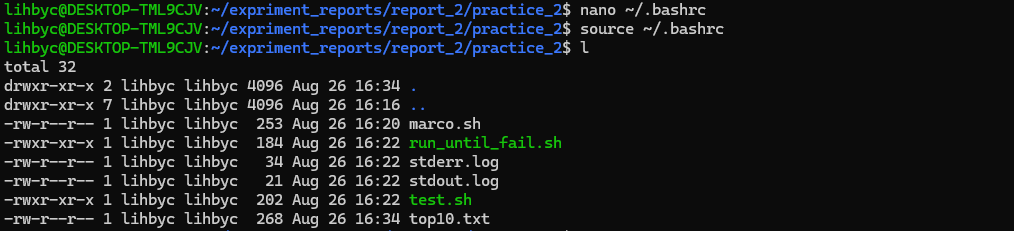
\includegraphics[width=0.8\textwidth]{p111.png}
\par
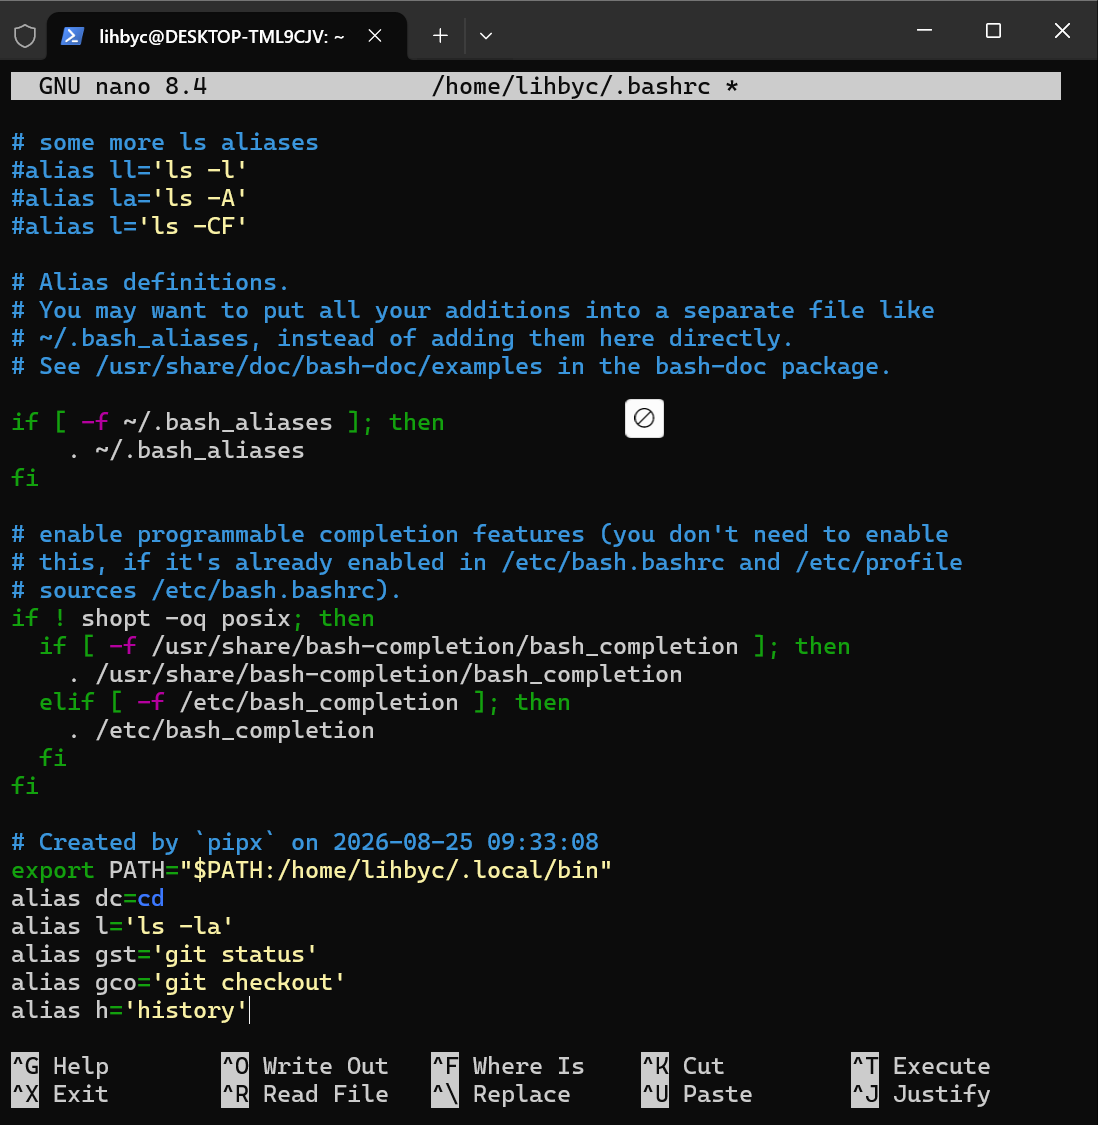
\includegraphics[width=0.8\textwidth]{p112.png}
\par

\textbf{结果：} 输入短别名即可执行相应长命令。

\textbf{解题感悟：} 合理的别名能显著缩短输入时间，但应保持易记，避免过度缩写导致遗忘。

\vspace{0.5cm}

\subsection*{练习12：使用 \texttt{strace} 跟踪系统调用}
\textbf{内容：} 使用 \texttt{strace} 跟踪 \texttt{ls -l} 的系统调用，观察其打开了哪些文件。

\textbf{操作步骤：}
\begin{enumerate}
    \item 执行 \texttt{strace -e trace=file ls -l} 仅跟踪文件操作。
    \item 或完整跟踪：\texttt{strace ls -l 2>\&1 | head -50}
    \item 分析输出，观察 \texttt{openat}, \texttt{read}, \texttt{write} 等调用。
\end{enumerate}

\par
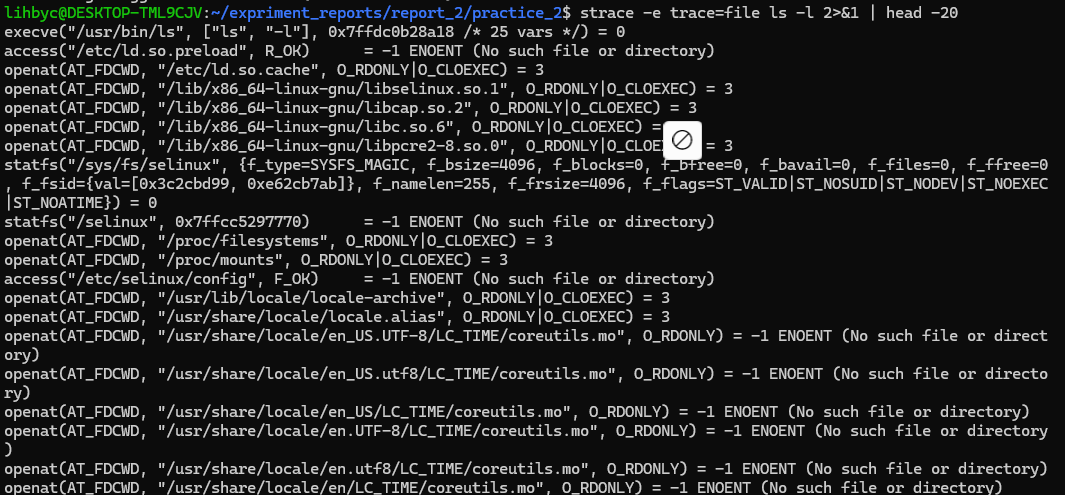
\includegraphics[width=0.8\textwidth]{p121.png}
\par
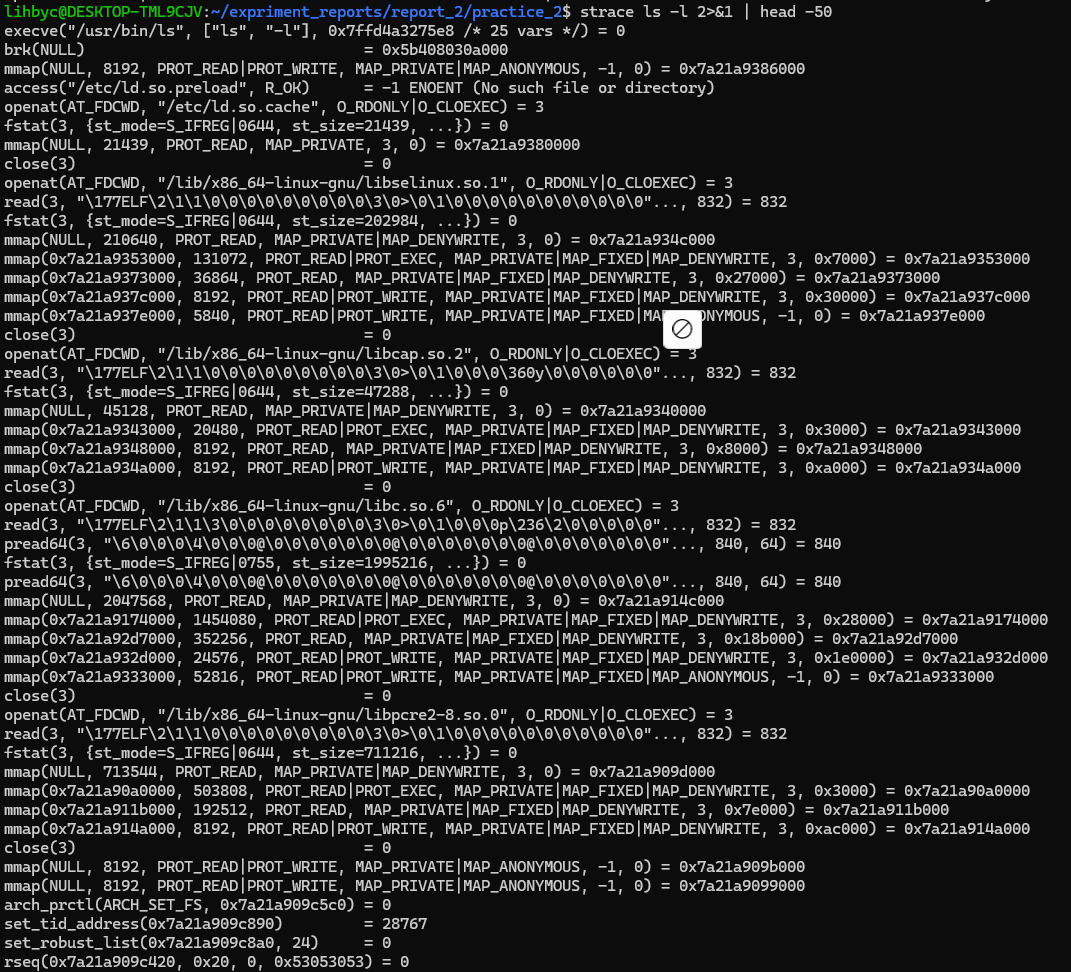
\includegraphics[width=0.8\textwidth]{p122.png}
\par
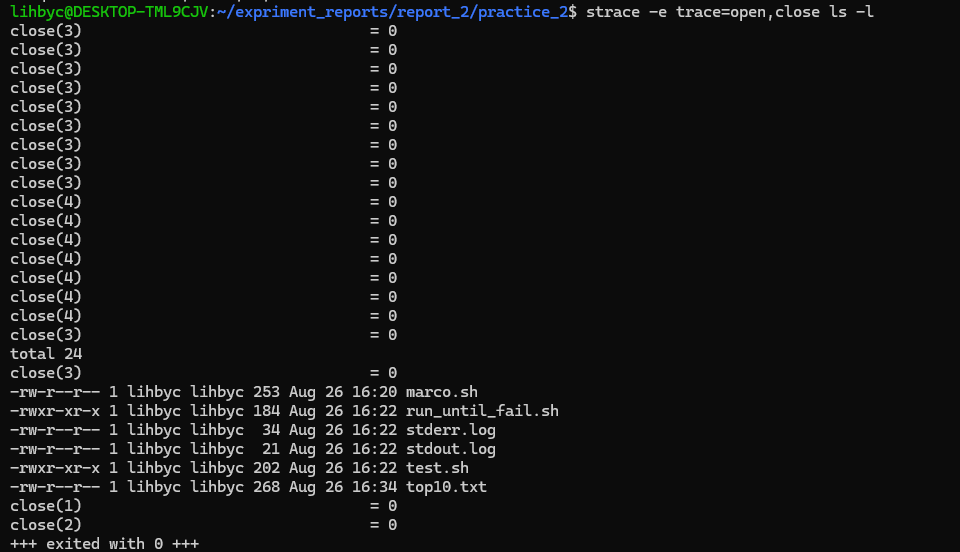
\includegraphics[width=0.8\textwidth]{p123.png}
\par
\textbf{结果：} 输出显示 \texttt{ls} 读取了当前目录、\texttt{/etc/ld.so.cache} 等动态链接库，以及终端的文件描述符。

\textbf{解题感悟：} \texttt{strace} 是诊断程序行为的有力工具，能揭示程序在底层与内核的交互，帮助排查权限、文件缺失等问题。

\end{document}
